\section{Metodi di iterazione funzionale}
Per trovare altri metodi, differenti da quello di bisezione, possiamo osservare che la nostra funzione
$f(x) = 0$ possiamo riscriverla in diversi modi:
\begin{align*}
	x = & x - f(x)              \\
	x = & x - \frac{f(x)}{h(x)}
\end{align*}
dove $h$ è una funzione definita sugli \emph{zeri} di $f$. Questo ci dice che il problema di trovare $x$ tale
che $f(x) = 0$ lo possiamo vedere come il problema nel trovare $x$ tale che
\[ x = g(x) \]
dove $g(x)$ potrebbe essere $x - f(x)$ oppure $x - \frac{f(x)}{h(x)}$. Posto in questi termini il problema non
è più quello di trovare gli zeri di $f$ ma diventa quello di trovare i \textbf{punti fissi} di $g$, ossia quei
punti $x$ di $g$ che si mandano in se stessi.

Questa equivalenza è interessante poiché ci permette di vedere il problema in questo modo
\[
	\begin{cases}
		x_0 \in [a, b] \\
		x_{k+1} = g(x_k)
	\end{cases}
\]
e possiamo dimostrare facilmente che se $g : \R \to \R$ è continua e
\[ \lim_{k \to +\infty} x_{k} = \alpha \]
allora $g(\alpha) = \alpha$, quindi $\alpha$ è un punto fisso di $g$ e uno zero di $f$.

\begin{example}
	Consideriamo l'equazione
	\[ \sqrt{x} - x = 0 \]
	Prima di tutto notiamo che la funzione è definita per $x \geq 0$ e poi, sviluppando l'equazione, possiamo
	scrivere
	\begin{align*}
		\sqrt{x} - x = & 0   \\
		\sqrt{x} =     & x   \\
		x =            & x^2 \\
		x^2 - x =      & 0   \\
		x (x - 1) =    & 0
	\end{align*}
	Ottenendo così le soluzioni $x = 0$ e $x = 1$. Notiamo però che l'equazione può essere scritta come
	\[ x = \sqrt{x} \]
	e quindi possiamo dire che
	\[ g_1(x) = \sqrt{x} \]
	Riconducendoci al sistema di prima possiamo scrivere
	\[ x_{k+1} = g_1(x_k) = \sqrt{x_k} \]
	prendendo un qualsiasi $x_0 \in \R^+$. Proviamo a capire a cosa converge la successione che calcoliamo.
	Prima di tutto disegnamo un grafico per la funzione $g_1$ e per la retta $x$
	\begin{center}
		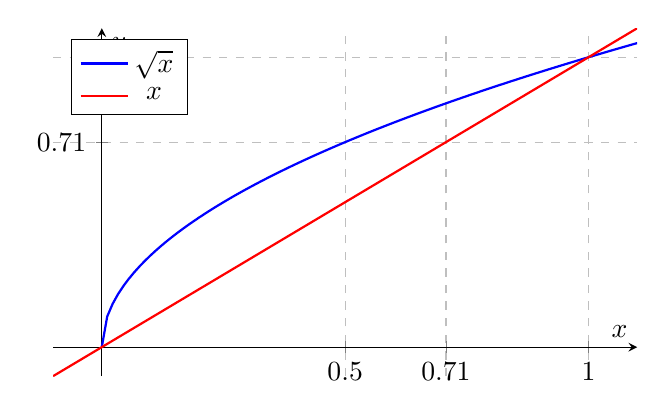
\begin{tikzpicture}
			\begin{axis}[
					font=\normalsize,
					width=9cm,
					height=6cm,
					axis lines = center,
					xlabel = $x$,
					ylabel = $y$,
					xtick = {1/2, sqrt(1/2), 1},
					ytick = {sqrt(1/2), 1},
					ymin = 0, ymax = 1,
					xmin = 0, xmax = 1,
					grid = both,
					grid style = dashed,
					legend pos = north west,
					enlargelimits
				]

				\addplot [
					domain=0:1.1,
					samples=100,
					thick,
					color=blue
				]
				{sqrt(x)};

				\addplot [
					domain=-0.1:1.1,
					samples=20,
					thick,
					color=red
				]
				{x};

				\legend{
					$\sqrt{x}$,
					$x$
				}
			\end{axis}
		\end{tikzpicture}
	\end{center}
	Scegliamo un $x_0$ compreso tra 0 e 1, supponiamo $\frac{1}{2}$, e proviamo a calcolare qualche $x_i$ per
	vedere come procede la successione. Come sappiamo per calcolare $x_1$ dobbiamo applicare a $x_0$ la nostra
	funzione $g_1$. Otteniamo quindi
	\begin{gather*}
		x_1 = \sqrt{x_0} = \sqrt{0.5} = 0.71 \\
		x_2 = \sqrt{x_1} = \sqrt{0.71} = 0.84
	\end{gather*}

	\begin{center}
		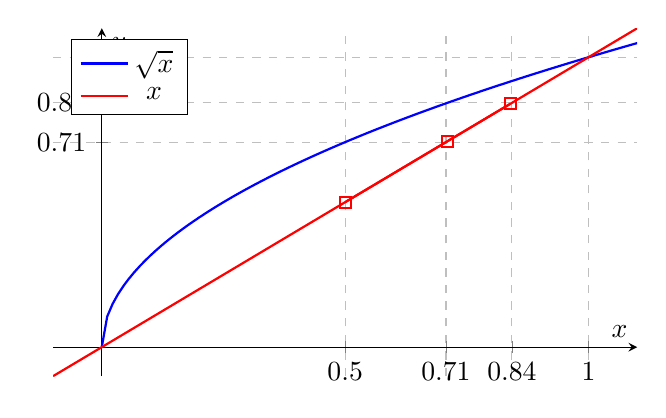
\begin{tikzpicture}
			\begin{axis}[
					font=\normalsize,
					width=9cm,
					height=6cm,
					axis lines = center,
					xlabel = $x$,
					ylabel = $y$,
					xtick = {1/2, sqrt(1/2), sqrt(0.71), 1},
					ytick = {sqrt(1/2), sqrt(0.71), 1},
					ymin = 0, ymax = 1,
					xmin = 0, xmax = 1,
					grid = both,
					grid style = dashed,
					legend pos = north west,
					enlargelimits
				]

				\addplot [
					domain=0:1.1,
					samples=100,
					thick,
					color=blue
				]
				{sqrt(x)};

				\addplot [
					domain=-0.1:1.1,
					samples=20,
					thick,
					color=red
				]
				{x};

				\addplot [
					domain=-0.1:1.1,
					samples=20,
					thick,
					color=red,
					mark=square
				]
				coordinates { (1/2, 1/2) (0.71, 0.71) (0.84, 0.84) };

				\legend{
					$\sqrt{x}$,
					$x$
				}
			\end{axis}
		\end{tikzpicture}
	\end{center}
	Andando avanti ci si accorge che se $0 < x_0 < 1$ allora $x_k$ tende a 1 per $k \to +\infty$. Se definiamo
	$x_0 > 1$ la situazione non cambia. Supponiamo di scegliere $x_0 = 1.1$, la successione che calcoliamo è
	la seguente
	\begin{gather*}
		x_1 = \sqrt{1.1} = 1.05  \\
		x_2 = \sqrt{1.05} = 1.02
	\end{gather*}
	Graficamente otteniamo questo tipo di successione
	\begin{center}
		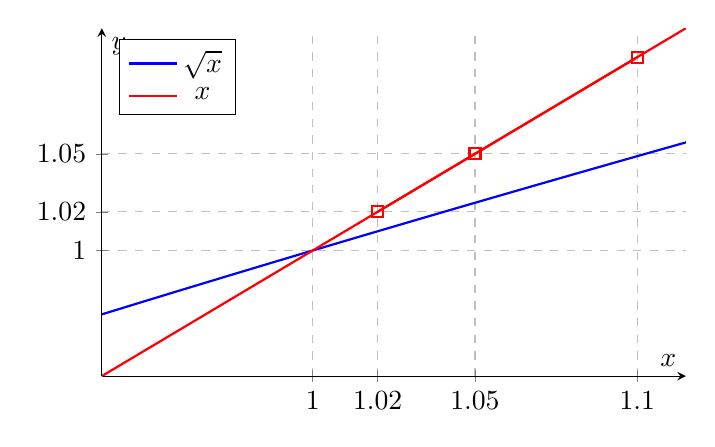
\begin{tikzpicture}
			\begin{axis}[
					font=\normalsize,
					width=9cm,
					height=6cm,
					axis lines = center,
					xlabel = $x$,
					ylabel = $y$,
					xtick = {1, 1.1, 1.05, 1.02},
					ytick = {1, 1.05, 1.02},
					ymin = 0.95, ymax = 1.1,
					xmin = 0.95, xmax = 1.1,
					grid = both,
					grid style = dashed,
					legend pos = north west,
					enlargelimits
				]

				\addplot [
					domain=0:1.2,
					samples=100,
					thick,
					color=blue
				]
				{sqrt(x)};

				\addplot [
					domain=0:1.2,
					samples=20,
					thick,
					color=red
				]
				{x};

				\addplot [
					domain=0.9:1.3,
					samples=20,
					thick,
					color=red,
					mark=square
				]
				coordinates { (1.1, 1.1) (1.05, 1.05) (1.02, 1.02) };

				\legend{
					$\sqrt{x}$,
					$x$
				}
			\end{axis}
		\end{tikzpicture}
	\end{center}
	Come possiamo vedere, anche in questo caso la successione converge a 1 per $k \to +\infty$. In generale
	possiamo osservare che, a meno che non scegliamo $x_0 = 0$, il metodo converge sempre a 1 anche se scegliamo
	$x_0$ molto vicino a 0. Se consideriamo un'equazione equivalente a $x = g_1(x)$, supponiamo $g_2(x) = x^2$
	e quindi
	\[ x = g_2(x) = x^2 \]
	calcoleremo la successione in questo modo
	\[ x_{k+1} = x_k^2 \]
	In questo caso, possiamo osservare come il metodo converga a 0 per $x_0 < 1$. Al contrario per $x_0 > 1$ il
	metodo diverge. Supponiamo ad esempio $x_0 = 0.5$ e facciamo due iterazioni
	\begin{gather*}
		x_1 = 0.5^2 = 0.25 \\
		x_2 = 0.25^2 = 0.625
	\end{gather*}
	Se invece scegliamo ad esempio $x_0 = 1.1$, dopo due iterazioni otteniamo
	\begin{gather*}
		x_1 = 1.1^2 = 1.21 \\
		x_2 = 1.21^2 = 1.46
	\end{gather*}
\end{example}

Questo esempio ci fa capire che abbiamo bisogno di un criterio per determinare delle condizioni di convergenza
indipendenti dalla scelta del punto iniziale.